% Generated by thesis/ch7/exp1/c4_units_figures.py -- do not edit by hand.
\begin{figure}[tbp]
  \centering
  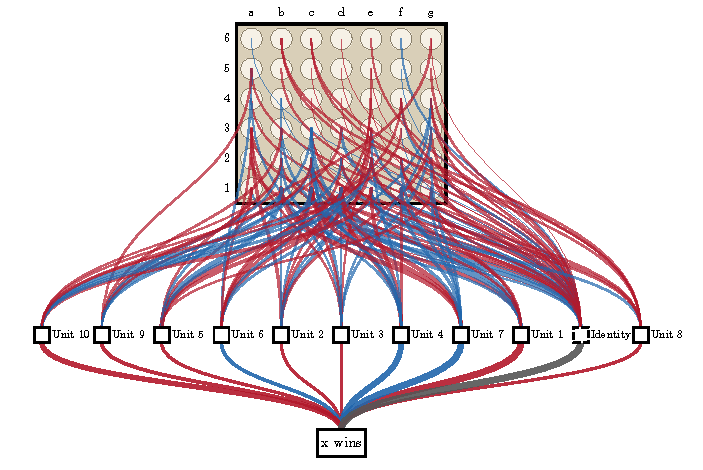
\includegraphics[width=\textwidth,height=0.8\textheight,keepaspectratio]{figures/ch7/c4-shared-board.pdf}
  \caption{Connect-4 cells network: board, hidden units, direct edges and output. Curves from the board to a unit: the unit's 8 inputs with the largest weights; to the identity node (dashed box): all 42 direct edges from the board to the output, collected by an identity node that passes their sum on unchanged. Blue where an x on the square raises x's chance of winning (through that unit, or directly), red where it lowers it; width by the size of that effect. Curves to the output: blue where the unit helps x when it fires, red where it hurts, grey from the identity node; width by the spread of the contribution.}
  \label{fig:ch7-c4-shared-board}
\end{figure}
